%!TEX root = ../../dokumentation.tex
%Umsetzung
\section{Image Preprocessing / Bildvorverarbeitung (Alex)} \label{sec:imagepreprocessing}
Bevor die geschriebenen Spielergebnisse für die Auswertung in die \textit{Support Vector Machine} gegeben werden können, müssen diese zuerst
für den \textit{Machine Learning}-Algorithmus vorbereitet werden. Dieser Prozess der Bildvorverarbeitung muss wiederum in weitere kleinere
Schritte aufgeteilt werden. Der Prozess beginnt mit einer Bilddatei, die von einem Nutzer in die Webapplikation hochgeladen wird. 
Die \textit{Support Vector Machine}, kann jedoch nur einzelne Bildausschnitte verarbeiten, die eine einzelne geschriebene Ziffer enthält.
Bei der Bildvorverarbeitung müssen demnach, die handschriftlich ausgefüllten Ziffern des Nutzers aus dem hochgeladenen Bild erkannt und
herausgeschnitten werden. Wie dies bewerkstelligt werden kann, wird im folgenden Kapitel herausgearbeitet.

Der Prozess bei Benutzung der Webapplikation kann folgendermaßen beschrieben werden. Der Nutzer füllt handschriftlich eine ausgedruckte Kniffel-Vorlage aus.
Die Vorlage enthält eine Tabelle mit Zeilen für die möglichen Würfelergebnisse und Spalten für die einzelnen Spiele. Diese Kniffel-Vorlage 
wird dann vom Nutzer abfotografiert und auf die Webseite hochgeladen. Damit die \textit{Support Vector Machine} die handschriftlichen Ziffern verarbeiten kann,
müssen die einzelnen Zellen der Tabelle, die die Spielergebnisse enthalten, aus dem hochgeladenen Bild ausgeschnitten werden. Eine Idee ist
ein Gitter über das Bild zu legen, das mit der Tabelle übereinstimmt, um so die einzelnen Zellen herauszuschneiden.

Ein Problem hierbei ist, dass das eingehende Bild von dem Nutzer abhängig ist. Die Qualität der Bilddatei und die Ausrichtung der darin abgebildeten 
Kniffel-Vorlage kann stark variieren. Es bestehen zwei Möglichkeiten dieses Problem zu lösen. Eine Lösung wäre es die Eckpunkte der Tabelle zu erkennen und 
dann das daraufzulegende Gitter anzupassen und daran auszurichten. Oder es wird da komplette Bild genommen und so ausgerichtet damit die abgebildete Tabelle
immer an derselben Position liegt. So kann immer dasselbe Gitter über das Bild gelegt werden und es muss nicht nochmals angepasst werden.
Bei der Umsetzung des Projektes fiel die Wahl auf den zweiten vorgestellten Lösungsansatz. Dieser Vorgang wird als \textit{Image Alignment} bezeichnet.

Der Prozess des \textit{Image Alignments} besteht aus drei verschiedenen Einzelschritten.
Zuerst werden zwei Bilder in den Algorithmus hineingegeben, die beide dasselbe Objekt zeigen, jedoch aus verschiedenen Blickwinkel beziehungsweise Perspektiven. 
Aus diesen beiden Eingangsbildern wird eine dann eine sogenannte Homografiematrix berechnet. Um diese Homografiematrix berechnen zu können gibt es verschiedene
Möglichkeiten. Häufig werden hierfür die \textit{Key Points} des Objektes betrachtet und wie die Position dieser Punkte auf den beiden Bildern miteinander korrespondieren. 
Zur Berechnung einer Homografiematrix können neben der \textit{feature}-basierten \textit{Key Point}-Korrespondez jedoch auch neuronale Netzwerke eingesetzt werden. 
Die Homografiematrix wird dann am Ende des \textit{Image Alignments} auf eines der Eingangsbilder angewandt und die Perspektive des Bildes damit so verzerrt, 
dass beide Bilder nun das abgebildete Objekt aus derselben Perspektive zeigen.\cite{rosebrock}

\begin{figure}[H]
	\centering
	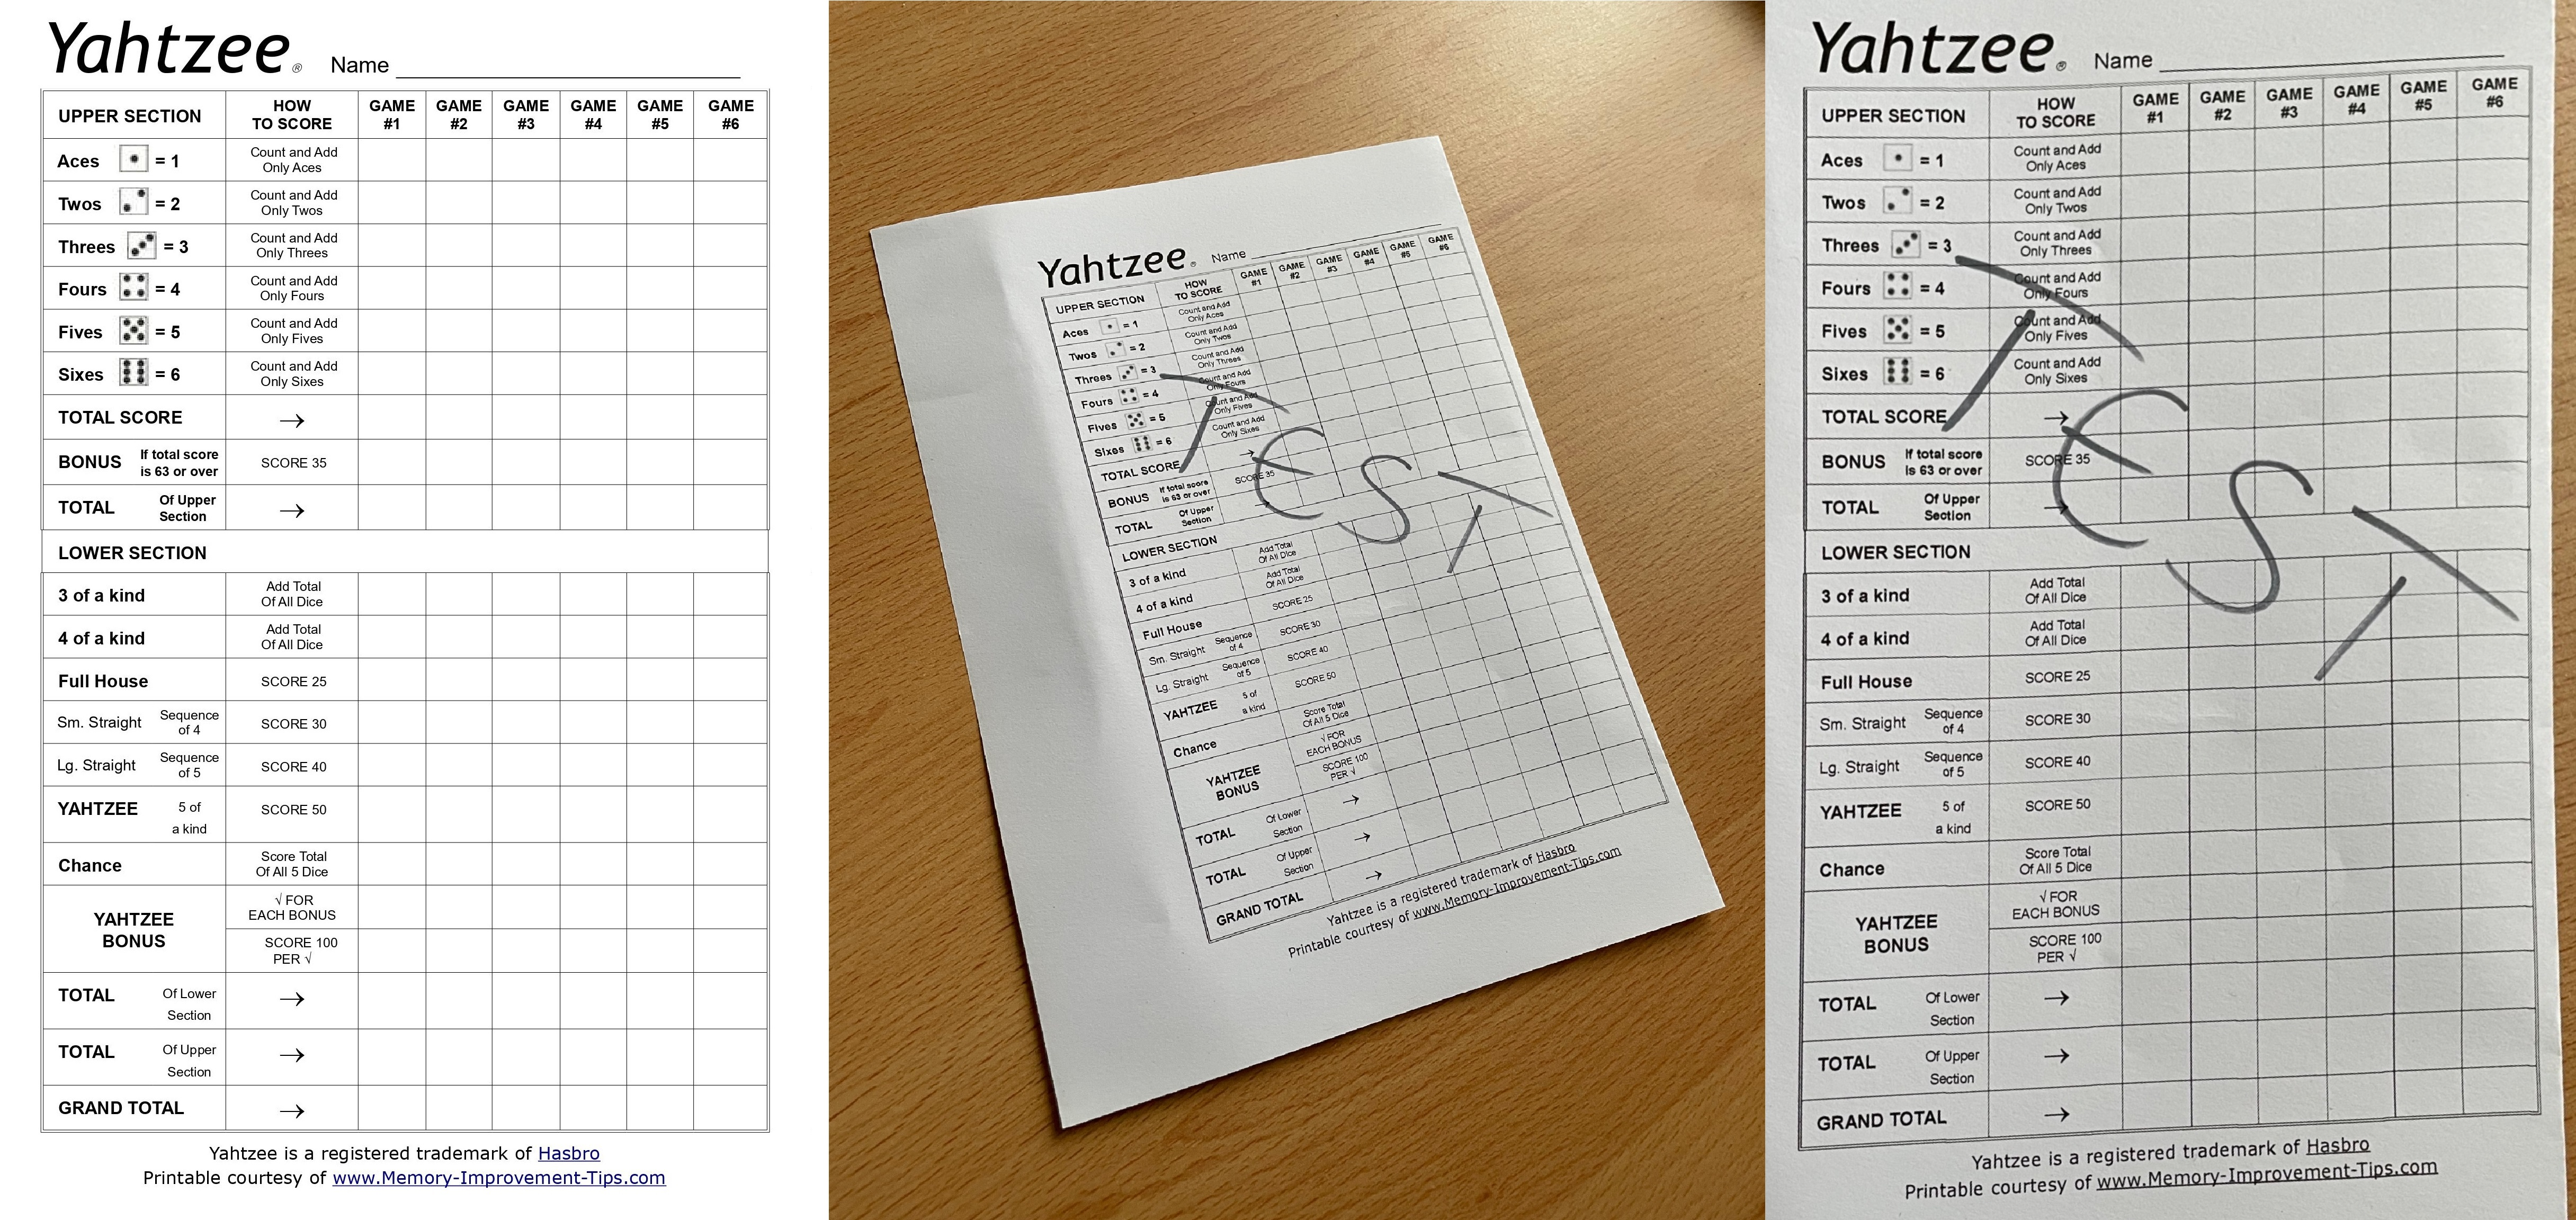
\includegraphics[width=\imgMed]{images/practice/image_alignment.jpg}
	\caption{\textit{Image Alignment}} 
	\label{fig:image_alignment}
\end{figure}

Abbildung \ref{fig:image_alignment} visualisiert das oben beschriebene \textit{Image Alignment}. Links ist die Yahtzee-Vorlage abgebildet, die auf der Webseite 
bereitgestellt wird und dann vom Nutzer heruntergeladen werden kann, der die Spielergebnisse einträgt. Die ausgefüllte Vorlage könnte dann so aussehen, wie das 
Bild in der Mitte, das das abfotografierte Formular zeigt. Zu guter Letzt sieht man auf der rechten Seite die abfotografierte Vorlage, die mit Hilfe von 
\textit{Image Alignment} so ausgerichtet wurde wie das linke Bild.

Für unsere Zwecke nutzen wir \textbf{OpenCV}, das bereits \textit{Key Point}-Erkennung von Bildern unterstützt. \textbf{OpenCV} sucht nach auffälligen Regionen,
den sogenannten \textit{Key Points}, innerhalb eines Eingangsbildes und extrahiert deren Deskriptoren. Mit diesen kann der umliegende Bereich um jeden 
\textit{Key Point} quantifiziert werden. Die \textit{Features} der \textit{Key Points} werden als 128-dimensionaler Vektor angegeben. Wenn 528 \textit{Key Points}
in dem Eingabebild gefunden wurden, haben wir jetzt 528 Vektoren, die alle 128-dimensional sind. Diese Vektoren können dann in einen Algorithmus wie RANSAC gegeben
werden, der die Korrespondenzen zwischen den \textit{Key Points} der beiden Bilder bestimmt.

\begin{figure}[H]
	\centering
	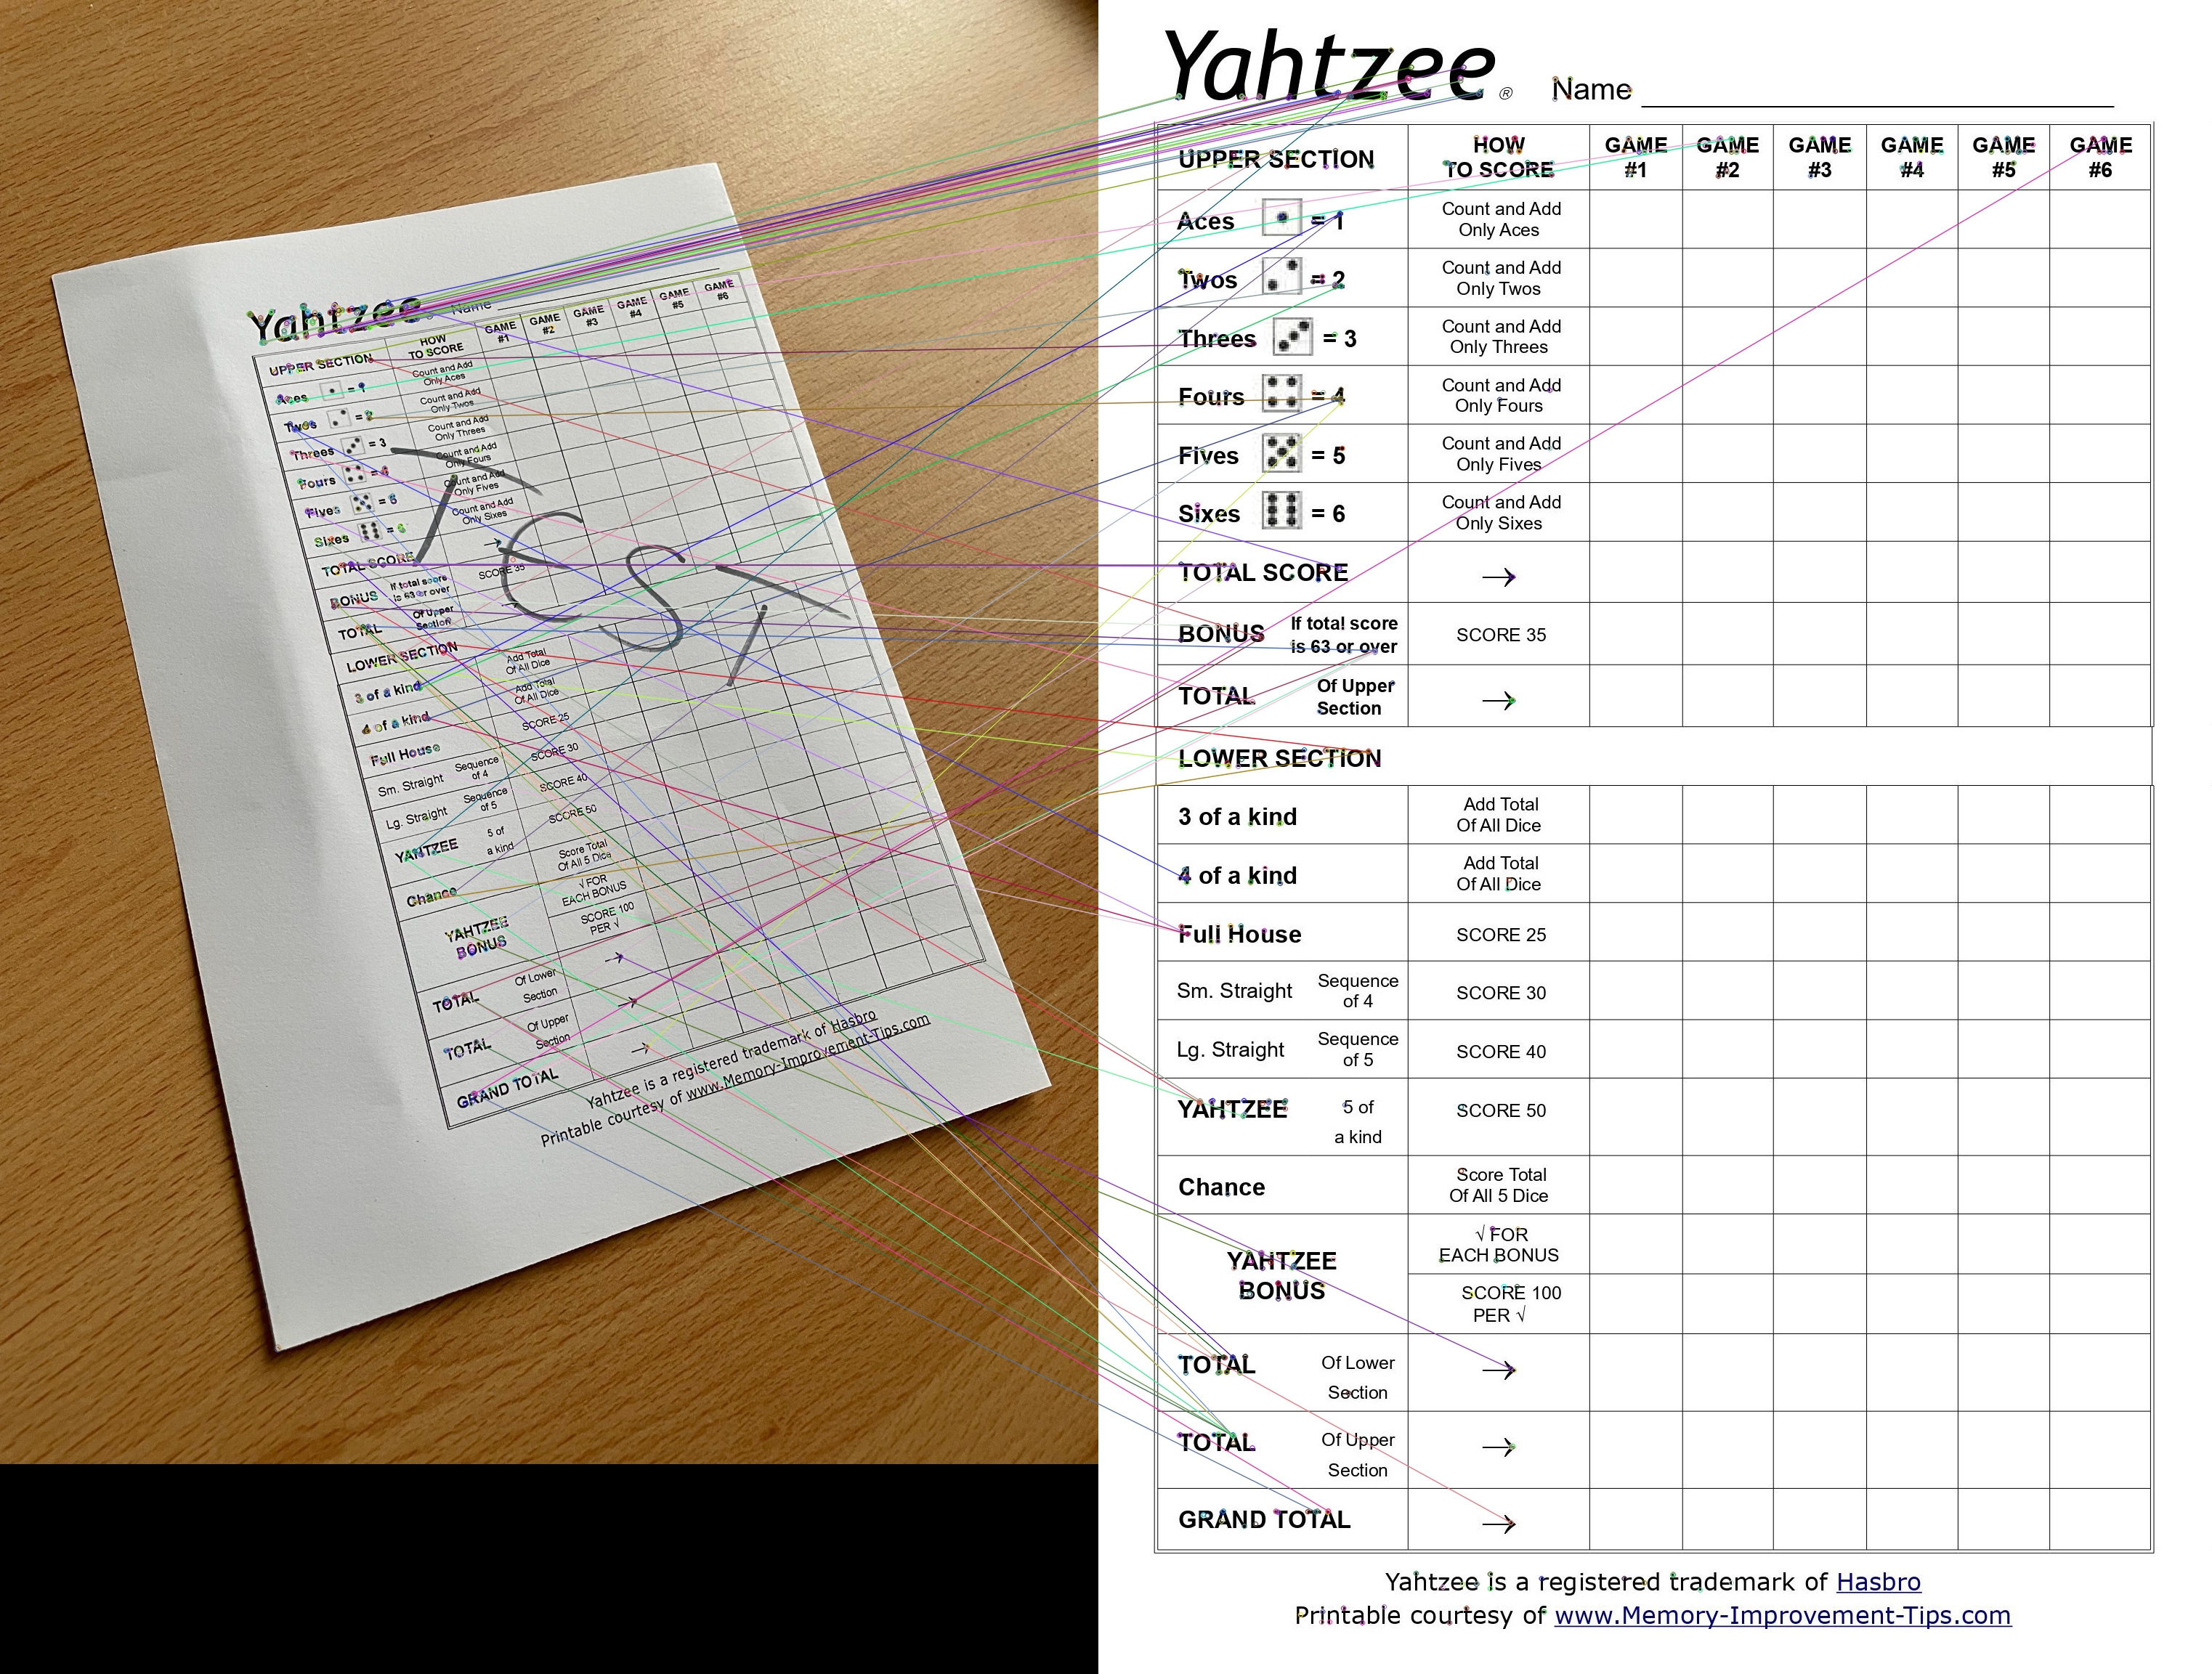
\includegraphics[width=\imgMed]{images/practice/correspondences.jpg}
	\caption{Korrespondenzen zwischen \textit{Key Points}} 
	\label{fig:correspondences}
\end{figure}

Wenn genug Übereinstimmungen zwischen den \textit{Key Points} der beiden Bilder existieren und ausreichend viele Korrespondenzen errechnet wurden, kann eine 
Homografiematrix mit den Ergebnissen erstellt werden. Diese Matrix beschreibt die perspektivische Verzerrung, die auf das Bild angewendet werden muss, um es
auszurichten. Sie gibt die Rotation, Verschiebung und Skalierung an, die das abfotografierte Bild genauso ausrichten wie das Vorlagebild. Mehr zur Homografie
ist \hyperref{https://docs.opencv.org/4.x/d9/dab/tutorial_homography.html}{}{}{hier} nachzulesen.\cite{rosebrock} Eine solche Homografiematrix sieht wie folgt aus:
\[s \begin{bmatrix} x^{'} \\ y^{'} \\ 1 \end{bmatrix} 
= H \begin{bmatrix} x \\ y \\ 1 \end{bmatrix} 
= \begin{bmatrix} h_{11} & h_{12} & h_{13} \\ h_{21} & h_{22} & h_{23} \\ h_{31} & h_{32} & h_{33} \end{bmatrix} 
\begin{bmatrix} x \\ y \\ 1 \end{bmatrix}\]
Viele der benötigten Funktionalitäten für das \textit{Image Alignment} werden bereits durch \textbf{OpenCV} bereitgestellt.
Die einzelnen Schritte müssen nun in \textbf{Python}-Code überführt werden. Der fertige Code, der in der Webapplikation verwendet wird, ist in \ref{lst:align_images}
abgebildet. Als Vorlage für den Code diente die Implementierung von \citeauthor{rosebrock}. Zuerst müssen das abfotografierte Bild und das Referenzbild
von \textbf{OpenCV} eingelesen werden. Vor dem eigentlichen \textit{Image Alignment} werden die beiden Bilder noch in ein Schwarzweiß-Format konvertiert.

Daraufhin werden mit Hilfe von \textbf{OpenCV} die ORB-\textit{Features} auf den beiden Eingangsbildern erkannt.
ORB steht hier für \textit{Oriented FAST and Rotated BRIEF}. Die ORB-\textit{Features} bestehen immer aus zwei Elementen: dem sogenannten 
\textit{Locator} sowie dem \textit{Descriptor}. Der \textit{Locator} identifiziert die \textit{Features}, die unabhängig von Verschiebung, Rotation und Skalierung
sind. Im \textit{Locator} werden die Koordinaten dieser Punkte abgespeichert. Der \textit{Descriptor} eines ORB-\textit{Features} codiert die äußeren Merkmale
des \textit{Features} als ein Array von Zahlen. Idealerweise haben die gleichen Punkte auf zwei verschiedenen Bildern auch denselben \textit{Descriptor}.
Die maximale Anzahl der zu erkennenden \textit{Features} werden mit dem Parameter \texttt{MAX\_FEATURES} festgelegt.

Danach werden die erkannten \textit{Features} der beiden Bilder einander anhand ihrer \textit{Descriptors} zugeordnet. 
Die Matches werden dann sortiert und die schlechten Matches herausgefiltert. Die globale Variable \texttt{GOOD\_MATCH\_PERCENT} legt fest wie viele
Matches nach dem Herausfiltern übrig bleiben sollen. In unserem Fall setzen wir die Variable auf 15\%. Zu Darstellungszwecken wird im Code eine
\texttt{matches.jpg} generiert, die die zuvor gefundenen Matches auf den beiden Bildern visualisiert. Mit dieser Codezeile wurde die Abbildung 
\ref{fig:correspondences} erstellt.

Als Nächstes wird die Positionierung der einzelnen Matches extrahiert und in einen \textbf{NumPy}-Array geschrieben. Mit Hilfe des RANSAC-Algorithmus wird
aus den Matches eine Homografiematrix berechnet. Diese Homografiematrix wird durch eine perspektivische Verzerrung auf das erste Bild angewendet.
Das neue Bild sowie die Homografiematrix werden zu guter Letzt von der Funktion zurückgegeben. Bild 1 hat nun dieselbe Perspektive auf das abgebildete Objekt,
wie die Vorlage in Bild 2.

\begin{minipage}{\textwidth}
	\begin{lstlisting}[language=Python, caption=Code für \textit{Image Alignment}, label=lst:align_images]
import cv2
import numpy as np

MAX_FEATURES, GOOD_MATCH_PERCENT = 500, 0.15

def align_images(im1, im2):
	# Bilder zu Schwarzweiss konvertieren
	im1Gray = cv2.cvtColor(im1, cv2.COLOR_BGR2GRAY)
	im2Gray = cv2.cvtColor(im2, cv2.COLOR_BGR2GRAY)

	# Erkennung der ORB-Features und Berechnung der Deskriptoren
	orb = cv2.ORB_create(MAX_FEATURES)
	keypoints1, descriptors1 = orb.detectAndCompute(im1Gray, None)
	keypoints2, descriptors2 = orb.detectAndCompute(im2Gray, None)

	# Matchen der Features
	matcher = cv2.DescriptorMatcher_create(cv2.DESCRIPTOR_MATCHER_BRUTEFORCE_HAMMING)
	matches = matcher.match(descriptors1, descriptors2, None)

	# Sortieren der Matches
	matches = sorted(matches, key=lambda x: x.distance, reverse=False)

	# Herausfiltern der schlechten Matches
	numGoodMatches = int(len(matches) * GOOD_MATCH_PERCENT)
	matches = matches[:numGoodMatches]

	# Zeichnen der Matches (zu Darstellungszwecken)
	imMatches = cv2.drawMatches(im1, keypoints1, im2, keypoints2, matches, None)
	cv2.imwrite("matches.jpg", imMatches)

	# Positionierung der Matches extrahieren
	points1 = np.zeros((len(matches), 2), dtype=np.float32)
	points2 = np.zeros((len(matches), 2), dtype=np.float32)
	for i, match in enumerate(matches):
		points1[i, :] = keypoints1[match.queryIdx].pt
		points2[i, :] = keypoints2[match.trainIdx].pt

	# Berechnung und Anwendung der Homografie
	h, mask = cv2.findHomography(points1, points2, cv2.RANSAC)
	height, width, channels = im2.shape
	im1Reg = cv2.warpPerspective(im1, h, (width, height))

	return im1Reg, h
	\end{lstlisting}
\end{minipage}

Die Eingangsbilder werden nun durch das \textit{Image Alignment} in dasselbe Format gebracht und zeigen danach die abgebildete Vorlage aus derselben Perspektive.
Da die Zellen der Tabelle aufgrund des \textit{Image Alignments} bis auf wenige Millimeter mit den Zellen der Vorlage übereinstimmen, können die Zellen einfach
anhand ihrer Koordinaten ausgeschnitten werden. Die minimalen Unterschiede, die das \textit{Image Alignment} nicht ausgleichen kann, können hierfür unberücksichtigt
bleiben.

Dafür wurde ein \textbf{Python}-Skript geschrieben, dass die Koordinaten der einzelnen Zellen der Tabelle aus der Vorlage enthält. Es erhält die Parameter \texttt{column} 
und \texttt{row} und gibt dann die dazugehörigen Werte der definierten Zelle zurück. Diese Rückgabewerte sind die x und y-Koordinate des linken oberen Punktes der
Tabellenzelle, sowie dessen Breite und Höhe. Diese vier Werte werden für den \texttt{crop()}-Befehl von \textbf{OpenCV} benötigt.

Mit Hilfe dieses Skriptes und \textbf{OpenCV} kann sehr einfach über die benötigten Spalten und Zeilen der Tabelle iteriert werden und die dazugehörige Zelle der 
Tabelle ausgeschnitten werden. Die ausgeschnittenen Tabellenzellen können jedoch noch nicht in den \textit{Machine Learning}-Algorithmus gegeben werden, da es sich immer
noch um mehrstellige Zahlen in der Zelle handeln könnte. Diese können noch nicht vom Algorithmus ausgewertet werden, da dieser nur Zahlen erkennen kann.
Wie mehrstellige Zahlen erfasst werden können, wird im darauffolgenden Kapitel zur Zahlenerkennung beantwortet.
